\section{Cripto-codificación caótica variante en el tiempo}
\label{sec:CodCaot}

En esta sección se presenta una nueva técnica para la criptocodificación de datos mediante una familia de mapas caóticos.
El diseño se basa en los mapas cuadráticos bidimensionales presentados en la sección \ref{ssecQMaps}, aprovechando su característica de modificar su atractor según los valores que tomen sus 12 coeficientes reales.
Para la implementación se utilizo aritmética de punto fijo con 19 bits.
Se realizaron simulaciones y el diseño en VHDL mediante el programa Quartus II v8.0 de ALTERA, para su posterior implementación en FPGA.

En los sistemas de comunicaciones y particularmente en los dedicados a la codificación para el control de error y encriptamiento de datos se usan técnicas derivadas de la teoría de señales.
Estas técnicas se aplican típicamente en la forma lineal debido a la simplicidad que ésto trae aparejado.
Además cada una se implementa algorítmicamente o físicamente como una entidad independiente.
Para cada sistema en particular se las elige con criterios de conveniencia práctica, y se las aplica en forma consecutiva o encadenada.
La teoría de los sistemas no lineales \cite{Strogatz1994,Lasota1994} aparece como un marco de trabajo ideal para ser utilizado en el contexto anteriormente mencionado.
La existencia de los sistemas caóticos, y la relación de estos con la aleatoriedad, o pseudo aleatoriedad, otorga una plataforma de diseño que hasta hoy se encuentra poco explotada.

En los últimos veinte años se han presentado diversos trabajos que emplean caos en los sistemas de comunicaciones, como por ejemplo el empleo de portadoras caóticas sincronizadas en las transmisiones analógicas \cite{Kocarev1995,Hidalgo2001}.
Si nos centramos en la representación discreta un referente muy importante es el excelente trabajo de Kozic et als. \cite{Kozic2006A,Kozic2006B} en el que se presenta una técnica de modulación empleando mapas caóticos unidimensionales lineales por tramos, la técnica consiste en la introducción del mensaje a codificar en el bit menos significativo de la secuencia generada.
Así, se obtiene una secuencia levemente alterada lo que impide que el sistema entre en ciclos periódicos.

En este trabajo se propone un grupo de atractores como generadores de señales pseudoaleatorias para realizar el proceso de codificación y encriptamiento.
El esquema de codificación se basa en la familia de mapas cuadráticos bidimensionales, cuyas salidas presentan comportamiento caótico, con distintos atractores conforme a los coeficientes que se empleen.
La idea es que cada palabra a codificar sea unívoca con un juego de coeficientes que serán parámetros de un mapa cuadrático bidimensional.
Como resultado de este procedimiento, la señal de salida son puntos pertenecientes a distintos atractores elegidos por la información a transmitir.

La ventaja de este método reside en que la estructura de toda la familia de mapas es única y común.
Modificándose solamente los coeficientes se consiguen atractores distintos.
Esta propiedad reduce y facilita la implementación en hardware.
Resultados preliminares obtenidos mediante simulaciones muestran que el sistema presenta una performance comparable a la obtenida en sistemas clásicos de encriptamiento, en cuanto a probabilidad de error y distancia mínima.

\subsection{Implementación}

Desde el punto de vista del esquema de codificación propuesto, estos mapas son muy atractivos por el hecho de contar con $12$ coeficientes para generar cada atractor.
Por lo tanto, las combinaciones posibles serán $N^{12}$, en donde $N$ es la cantidad de símbolos posibles según la aritmética utilizada.
En nuestro caso empleamos una aritmética de $19$ bits expresados en complemento a $2$ con aritmética de punto fijo, con $1$ bit de signo, $3$ bits de parte entera y $15$ bits de parte decimal.
Esta aritmética limita y discretiza el plano $xy$ que queda delimitado por $\Delta x=4$, $-\Delta x=-4$, $\Delta y=4$,$-\Delta y=-4$, como puede verse en la figura \ref{fig:atractores}.
Estas limitaciones al plano de atracción tienen como consecuencia dos cuestiones a tener en cuenta:
\begin{itemize}
    \item
        Debido a que los coeficientes se generan con la misma aritmética que las variables, nos encontramos con $N=2^{19}$ valores posibles para cada coeficiente, lo que arroja $\left(2^{19}\right)^{12}\cong4,3^{68}$ combinaciones posibles de coeficientes para generar distintos atractores.
    \item
        En cuanto a las trayectorias de los atractores sobre el plano discretizado, éstas se tornan periódicas debido a la discretización.
\end{itemize}

No todos los juegos de coeficientes generan atractores caóticos contenidos en el plano dado por la aritmética utilizada.
Aunque esto no sería problema para la codificación/decodificación, se eligieron los coeficientes de modo que se generen atractores contenidos en el plano a modo de validación visual.

Dada la naturaleza de los mapas caóticos, un punto muy lejano a la zona de atracción puede hacer que el punto calculado para la próxima iteración diverja, por lo tanto las condiciones iniciales deben ser normalizadas antes de cambiar al mapa siguiente.
Para solucionar este problema se utiliza la siguiente estrategia:
\begin{itemize}
	\item Primero se define el plano mínimo que contiene al atractor.
	Para identificarlo se simularon los mapas mediante Quartus generando secuencias de salida lo suficientemente largas como para verificar la periodicidad.
	Luego se analizó este vector de datos con Matlab buscando los valores extremos en cada una de las variables: $X1_{max}$, $X1_{min}$, $Y1_{max}$, $Y1_{min}$.
	Estos límites delimitan al plano mínimo que contiene al atractor.
	La normalización dada por la ecuación \ref{eq:norm_salida} se aplica a la salida $\left(x,y\right)$ para mapear este plano minimo a todo el plano delimitado por la aritmética utilizada de dimensiones $\Delta x$, $-\Delta x$, $\Delta y$, $-\Delta y$.
	\item Segundo, se halla el plano máximo que contiene las condiciones iniciales que hacen que no diverja la solución sino que genere el atractor.
	Para esto se realizó un programa en Matlab que genera los atractores desde todas las condiciones iniciales del plano delimitado y discretizado por la aritmética utilizada, a continuación se marcan todos los puntos que generan trayectorias divergantes o bien convergentes a un punto fijo. 
	Este proceso genera la zona de condiciones iniciales factible para generar atractores, nuevamente se identificaron los valores máximos y mínimos del área rectangular máxima que contenga todos sus puntos como condiciones iniciales factibles $X2_{max}$, $X2_{min}$, $Y2_{max}$, $Y2_{min}$. 
	La normalización dada por la ecuación \ref{eq:norm_entrada} se aplica a la entrada de condiciones iniciales $\left(x_{n-1},y_{n-1}\right)$ para mapear todo el plano de dimensiones $\Delta x$, $-\Delta x$, $\Delta y$ y $-\Delta y$ al de condiciones iniciales factibles.
\end{itemize}
%
\begin{eqnarray}\label{eq:norm_salida}
x_{1norm}&=& a_{1x} x+b_{1x} \nonumber\\
y_{1norm}&=& a_{1y} y+b_{1x} \nonumber\\
a_{1x}&=& \frac{2\Delta x}{x1_{max}-x1_{min}} \nonumber\\
a_{1y}&=& \frac{2\Delta y}{y1_{max}-y1_{min}} \nonumber\\
b_{1x}&=& -\frac{x1_{max}-x1_{min}}{2} \nonumber\\
b_{1x}&=& -\frac{y1_{max}-y1_{min}}{2}
\end{eqnarray}
%
\begin{eqnarray}\label{eq:norm_entrada}
x_{1norm}&=& a_{2x} x+b_{2x} \nonumber\\
y_{1norm}&=& a_{2y} y+b_{2x} \nonumber\\
a_{2x}&=& \frac{x2_{max}-x2_{min}}{2\Delta x} \nonumber\\
a_{2y}&=& \frac{y2_{max}-y2_{min}}{2\Delta y} \nonumber\\
b_{2x}&=& \frac{x2_{max}-x2_{min}}{2} \nonumber\\
b_{2x}&=& \frac{y2_{max}-y2_{min}}{2}
\end{eqnarray}

El problema de la existencia de puntos fijos para cierto conjunto de coeficientes y condiciones iniciales queda salvado al perturbar continuamente al atractor actual con valores afectados por la información.

Se generó un circuito en VHDL con un total de $16$ juegos de parámetros seleccionables con la palabra de entrada de $4$ bits que se desea encriptar.
Esta palabra multiplexa estos coeficientes y alimenta un oscilador que calcula la próxima iteración de datos, además, este circuito almacena la salida del oscilador y la realimenta como ``condición inicial" para calcular la iteración siguiente (Fig. \ref{fig:generador}).
Como resultado de este proceso, la salida encriptada resulta ser el oscilador actual seleccionado por la palabra de entrada perturbado por la historia de los mapas seleccionados por las entradas anteriores.
Este circuito de dos bloques se encarga de generar los atractores, por lo que se lo llama ``generador de atractores".

Para la primer iteración, las condiciones iniciales son $(x;y)=(0.1;0.1)$ para cualquiera de los atractores.
%
\begin{figure}
    \centering
    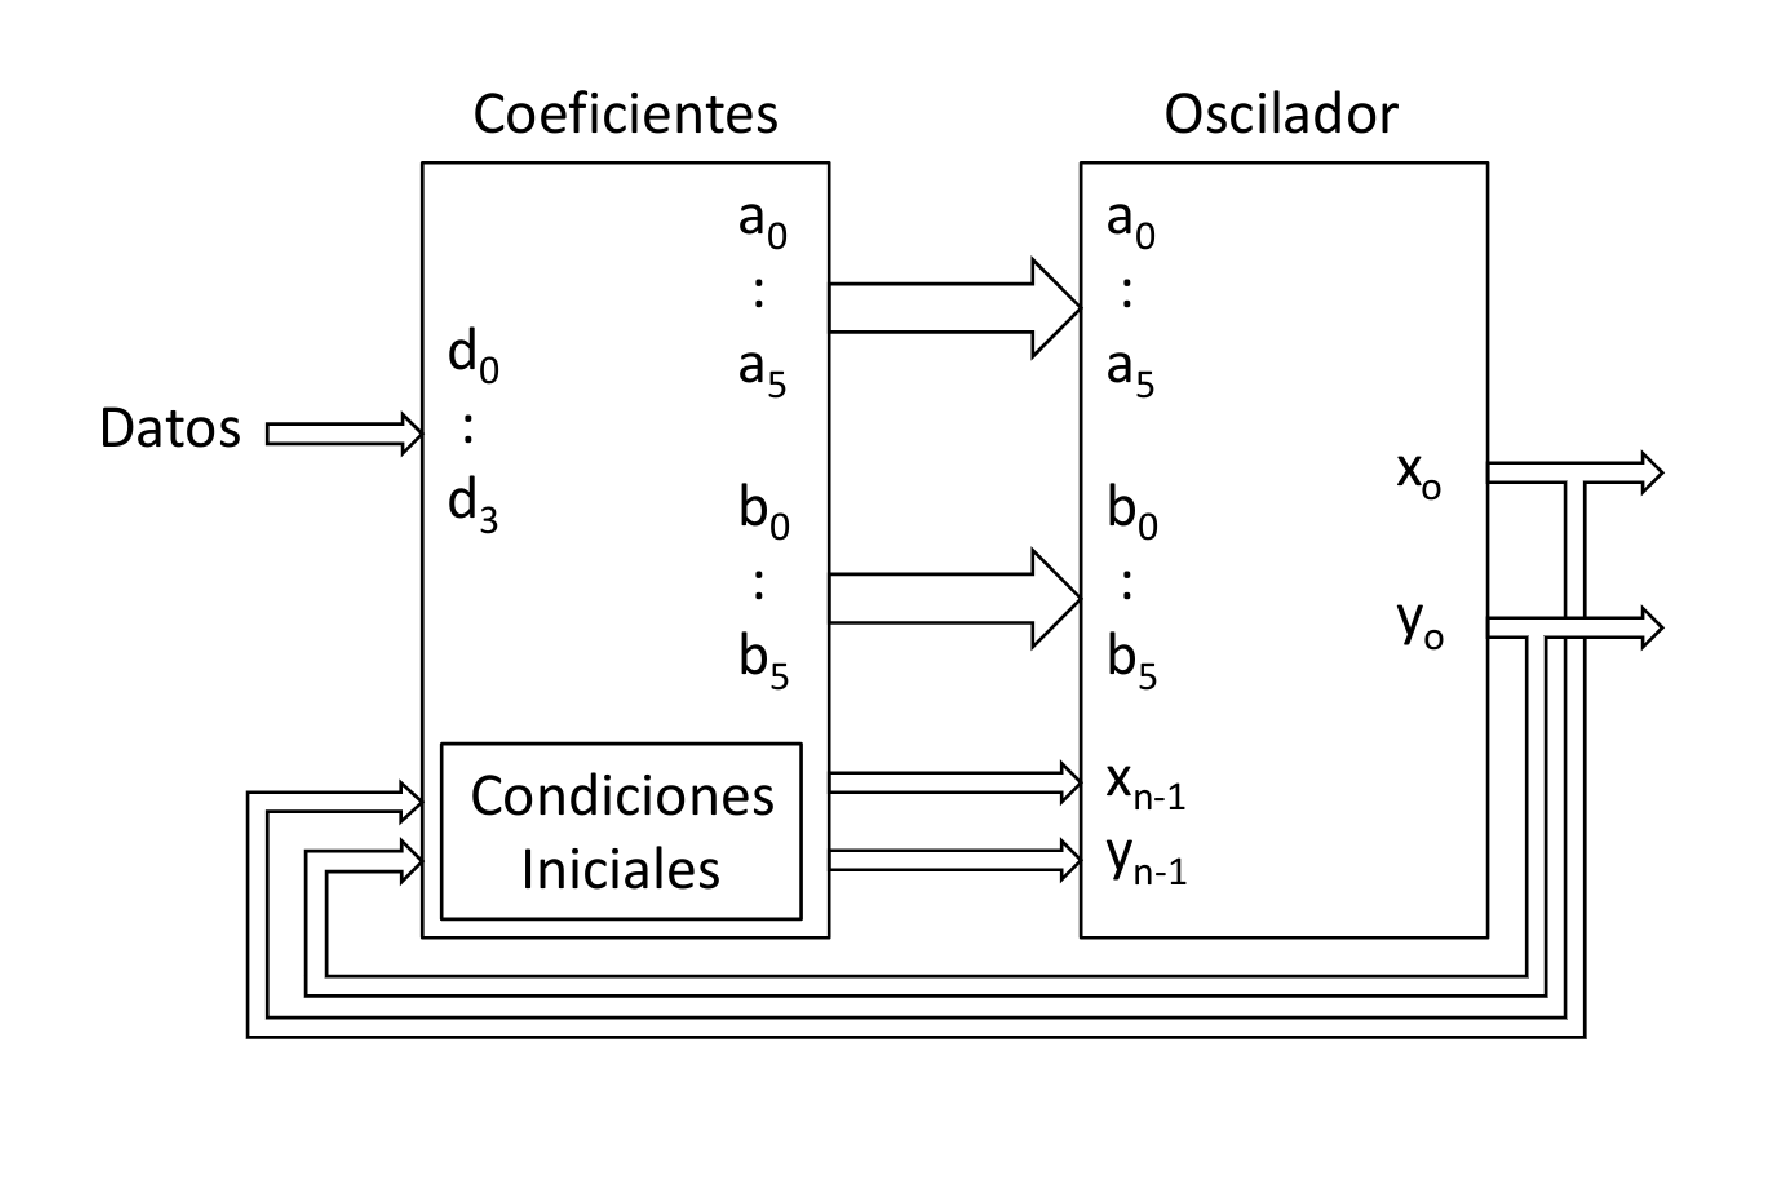
\includegraphics[width=0.7\columnwidth]{Fig1.pdf}\\
    \caption{Generador de atractores.}\label{fig:generador}
\end{figure}

\subsubsection{Codificador}
El bloque del Codificador consiste en circuito generador y acondicionamiento de la salida.
Para codificar una palabra de cuatro bits de entrada se generan los valores de $x$ e $y$ con el circuito generador correspondiente a esta palabra y se los concatena en un circito posterior formando un vector $[x:y]$ (Fig. \ref{fig:codificador}).
De esta forma cada palabra de información a ser enviada será representada por la salida $xy$  del oscilador del atractor correspondiente, por lo tanto una palabra a codificar no se corresponderá con una palabra codificada, dos palabras iguales generarán dos salidas distintas.
%
\begin{figure}
    \centering
    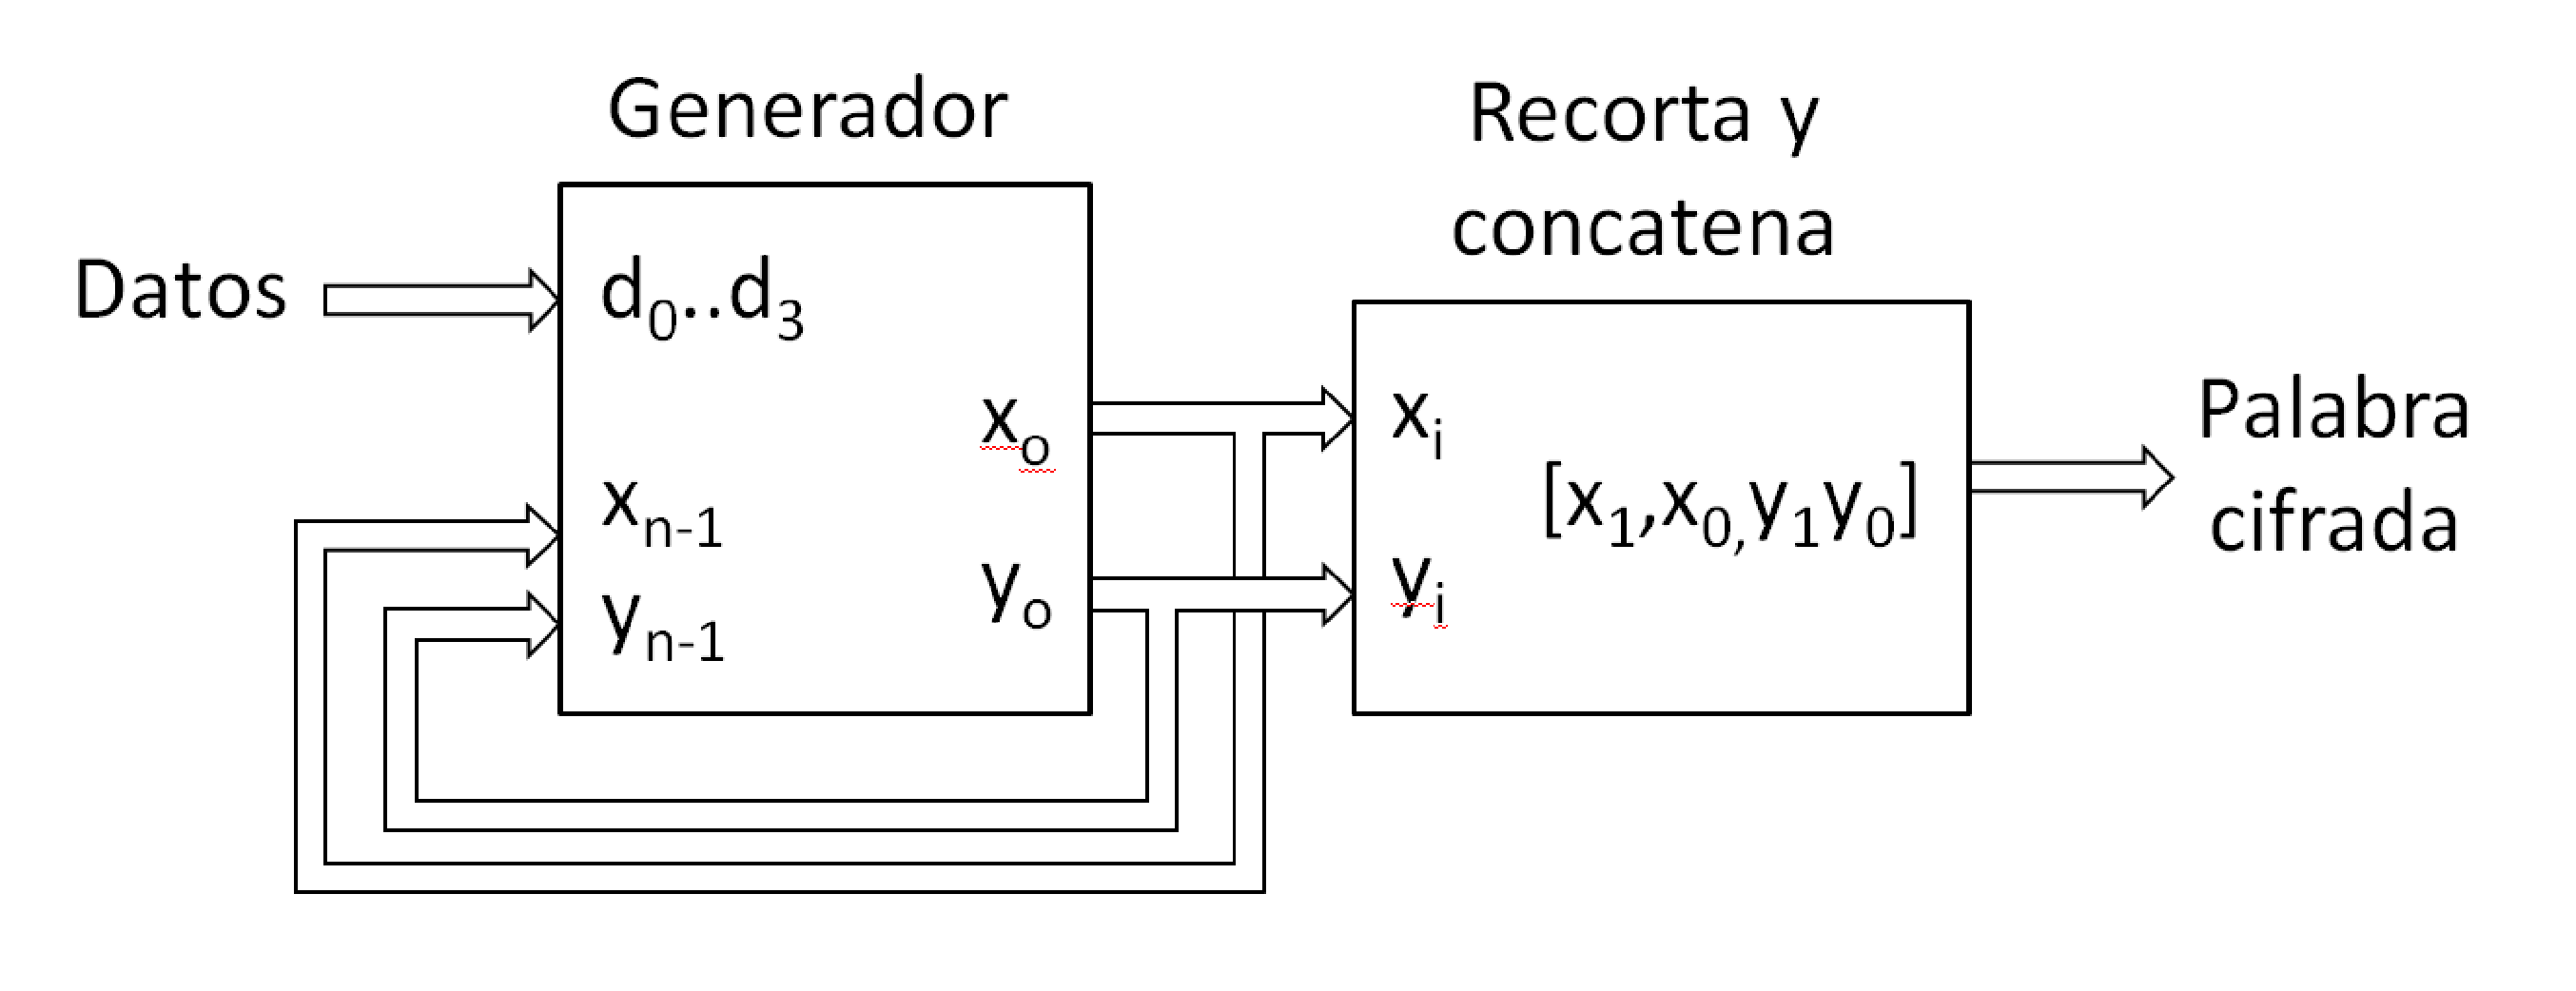
\includegraphics[width=0.8\columnwidth]{Fig2.pdf}\\
    \caption{Codificador.}\label{fig:codificador}
\end{figure}

\subsubsection{Decodificador}

Un segundo circuito generador de atractores funciona en el decodificador generando las $16$ palabras posibles para la próxima iteración.
Luego, se ingresan todas estas posibles palabras cifradas junto con la que se desea decodificar a un comparador que aplica una XOR a la palabra ingresada contra todas las palabras posibles generadas localmente para decodificarla.
La salida de este circuito es la palabra decodificada (Fig. \ref{fig:decodificador}).
%
\begin{figure}\
    \centering
    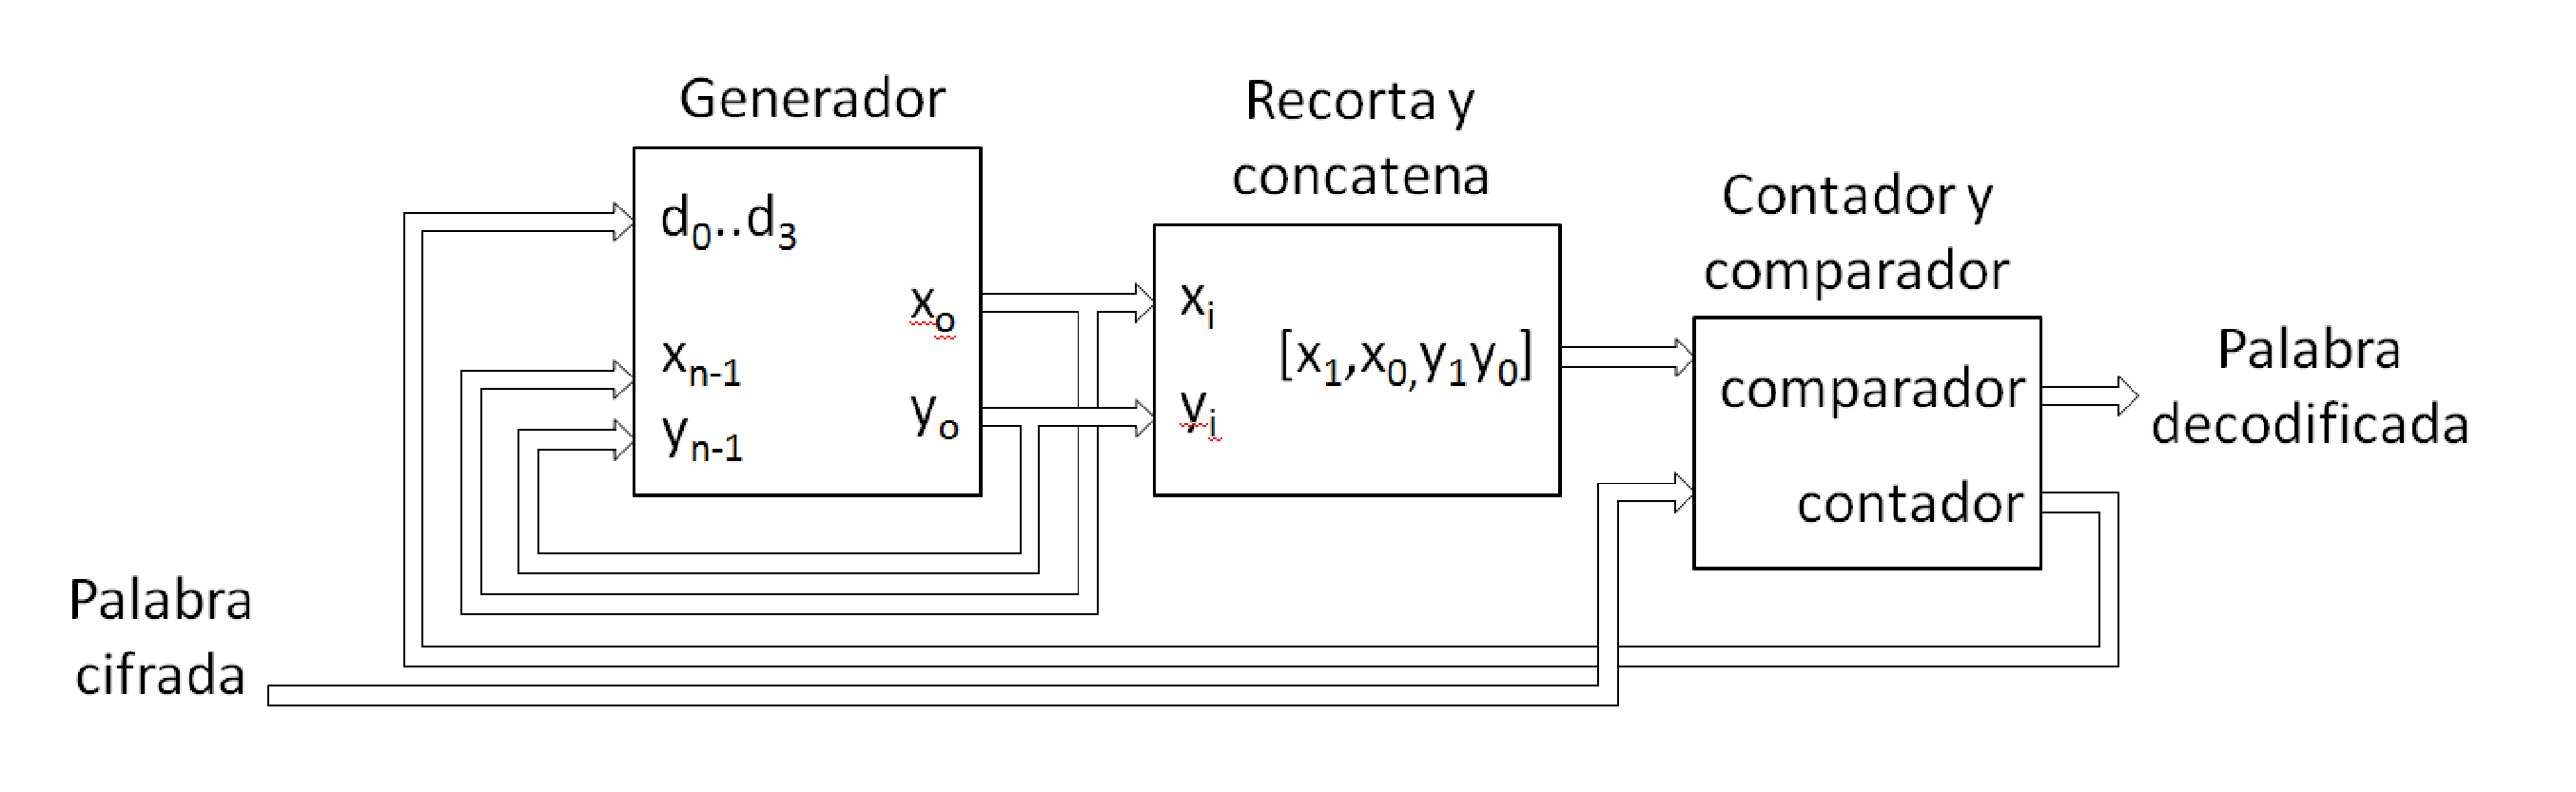
\includegraphics[width=0.95\columnwidth]{Fig3.pdf}\\
    \caption{Decodificador.}\label{fig:decodificador}
\end{figure}

\subsection{Resultados}

Se realizó un primer esquema del diseño mediante la herramienta Quartus II v8.0 de ALTERA, para implementar el sistema en una FPGA \emph{Altera Cyclone III EP3C120}.

Se obtuvieron resultados preliminares de simulaciones realizadas mediante el programa Matlab y mediante simulaciones con el programa Quartus de Altera, estas últimas tienen en cuenta el empleo de la precisión finita elegida para representar los valores.

En la Fig. \ref{senal} se pueden ver las salidas del bloque generador para una transmisión de los datos [1,2,3,2,3,3,1,3,1,3,1].
En este caso se mantiene el dato a enviar durante $100$ ciclos con el objetivo de que sea visible en la figura, en el sistema real cada oscilador codifica una palabra de información en cada iteración.
Aqui puede observarse que el sistema cambia el atractor generado según los coeficientes que dependen de la entrada de información a transmitir.
%
\begin{figure}
	\centering
	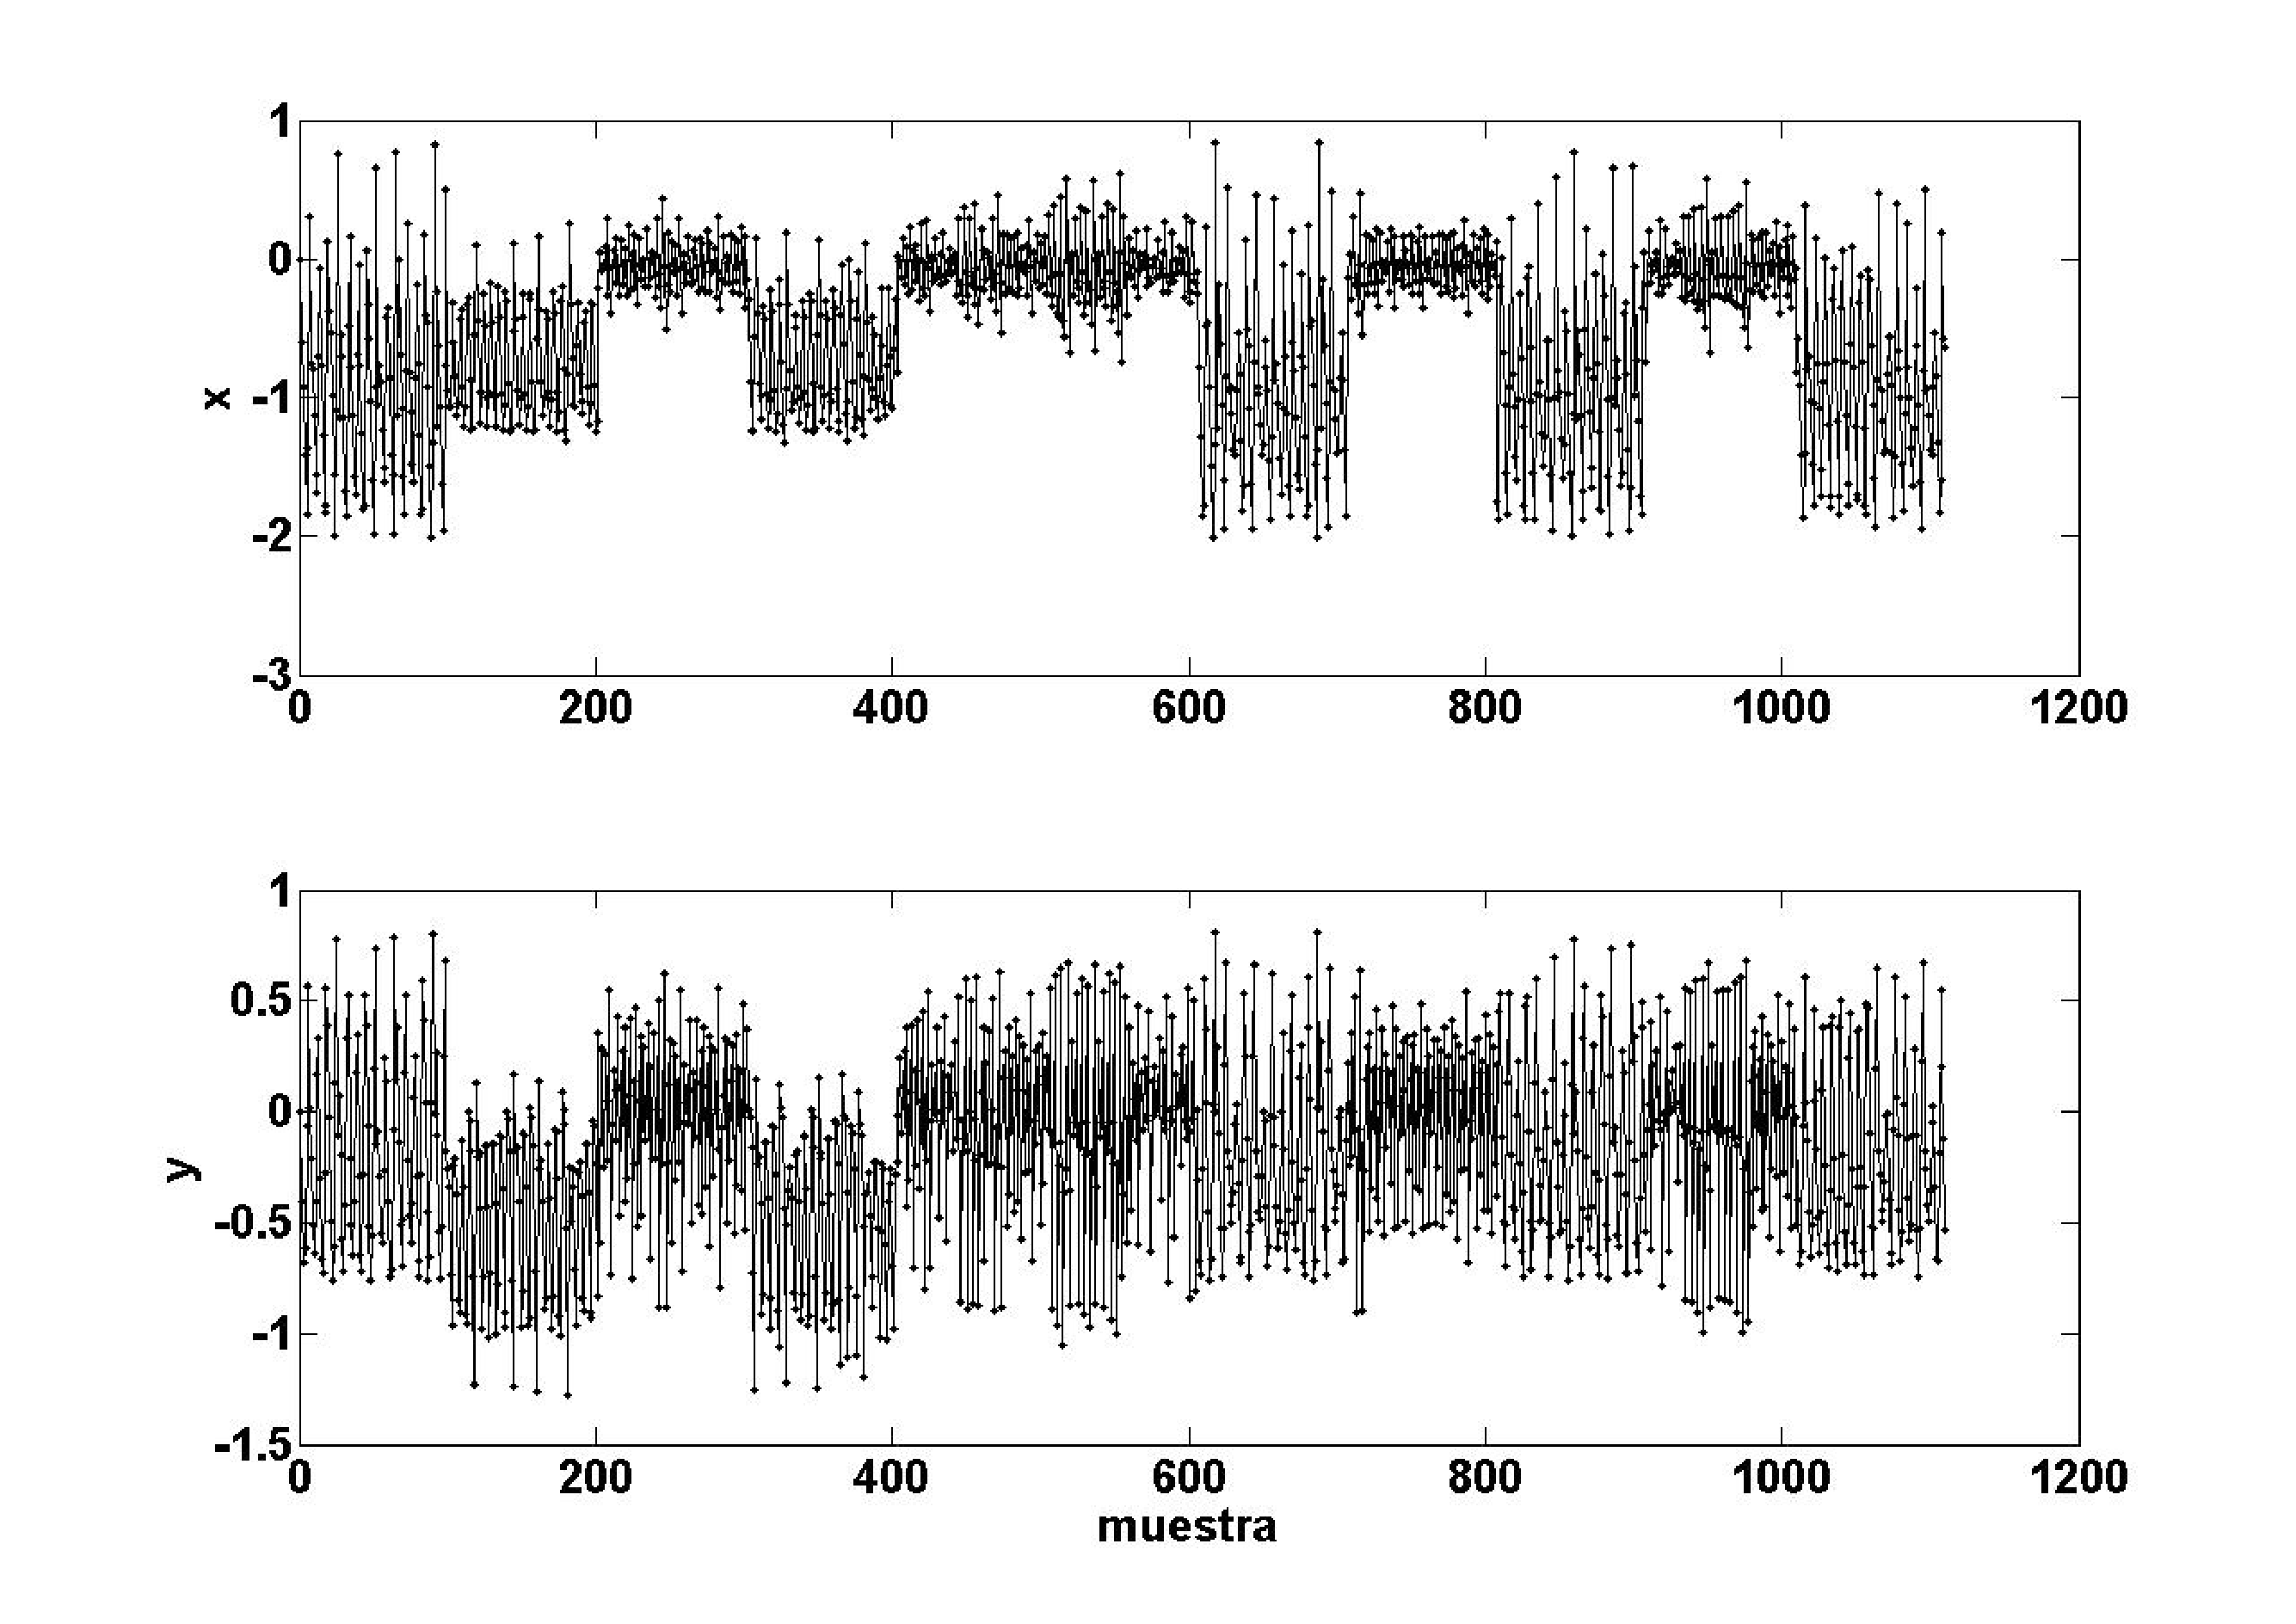
\includegraphics[width=1\columnwidth]{senalent.pdf}\\
	\caption{Señales a transmitir.}\label{senal}
\end{figure}